\documentclass[12pt,a4paper]{article}

% ─── Page Layout ───────────────────────────────────────────────────────────────
\usepackage[a4paper, margin=0.8in, headheight=14pt]{geometry}

% ─── Fonts (XeLaTeX) ───────────────────────────────────────────────────────────
\usepackage{fontspec}
\usepackage{unicode-math}
\setmainfont{TeX Gyre Pagella}
\setmonofont[Scale=0.88]{TeX Gyre Cursor}
\setmathfont{Latin Modern Math}

% ─── Packages ──────────────────────────────────────────────────────────────────
\usepackage{xcolor}
\usepackage{colortbl}
\usepackage{titlesec}
\usepackage{enumitem}
\usepackage{tabularx}
\usepackage{longtable}
\usepackage{booktabs}
\usepackage{array}
\usepackage{amsmath}
\usepackage{tikz}
\usetikzlibrary{shapes.geometric, arrows.meta, positioning, calc, fit, decorations.pathreplacing, patterns}
\usepackage{tcolorbox}
\tcbuselibrary{skins, breakable}
\usepackage{hyperref}
\usepackage{fancyhdr}
\usepackage{graphicx}
\usepackage{microtype}
\hyphenpenalty=10000
\exhyphenpenalty=10000
\sloppy
\usepackage{caption}
\usepackage{setspace}
\usepackage{multirow}
\usepackage{tocloft}

% ─── Q&A helper ────────────────────────────────────────────────────────────────
\newcommand{\Q}[1]{\textbf{#1}\par\noindent\ignorespaces}

% ─── Colour Palette ────────────────────────────────────────────────────────────
\definecolor{myred}{RGB}{196,30,58}
\definecolor{mydark}{RGB}{30,30,50}
\definecolor{mygreen}{RGB}{14,120,80}
\definecolor{myteal}{RGB}{0,130,140}
\definecolor{myamber}{RGB}{180,100,0}
\definecolor{mypurple}{RGB}{100,30,160}
\definecolor{mygray}{RGB}{246,247,249}
\definecolor{mgframe}{RGB}{180,185,200}
\definecolor{watermark}{RGB}{145,150,170}
\definecolor{hdrred}{RGB}{250,232,235}
\definecolor{hdrgreen}{RGB}{220,244,233}
\definecolor{hdrteal}{RGB}{220,242,244}
\definecolor{hdramber}{RGB}{253,242,215}
\definecolor{hdrpurple}{RGB}{238,228,255}
\definecolor{hdrgray}{RGB}{238,240,245}

% ─── Section Formatting ────────────────────────────────────────────────────────
\titleformat{\section}
  {\large\bfseries\color{myred}}{\thesection.}{0.5em}{}
  [\vspace{1pt}{\color{myred}\rule{\linewidth}{0.8pt}}]
\titleformat{\subsection}
  {\normalsize\bfseries\color{myteal}}{\thesubsection}{0.5em}{}
\titlespacing*{\section}{0pt}{18pt}{7pt}
\titlespacing*{\subsection}{0pt}{11pt}{4pt}

% ─── Paragraph ─────────────────────────────────────────────────────────────────
\setlength{\parindent}{0pt}
\setlength{\parskip}{4pt}

% ─── TOC Styling ───────────────────────────────────────────────────────────────
\renewcommand{\cfttoctitlefont}{\large\bfseries\color{myred}}
\renewcommand{\cftaftertoctitle}{\par\noindent{\color{myred}\rule{\linewidth}{0.8pt}}}
\setlength{\cftbeforetoctitleskip}{0pt}
\setlength{\cftaftertoctitleskip}{6pt}
\renewcommand{\cftsecfont}{\normalsize\bfseries\color{mydark}}
\renewcommand{\cftsecpagefont}{\normalsize\bfseries\color{mydark}}
\renewcommand{\cftsecleader}{\cftdotfill{\cftdotsep}}
\setlength{\cftbeforesecskip}{7pt}
\renewcommand{\cftsubsecfont}{\small\color{mydark}}
\renewcommand{\cftsubsecpagefont}{\small\color{mydark}}
\setlength{\cftbeforesubsecskip}{3pt}
\setlength{\cftsubsecindent}{1.4em}

% ─── Table helpers ─────────────────────────────────────────────────────────────
\renewcommand{\arraystretch}{1.45}
\setlength{\tabcolsep}{6pt}
\arrayrulecolor{mydark}
\newcolumntype{B}[1]{>{\small\bfseries\raggedright\arraybackslash}m{#1}}
\newcolumntype{Y}{>{\small\raggedright\arraybackslash}X}
\renewcommand{\tabularxcolumn}[1]{m{#1}}

% ─── Header / Footer ───────────────────────────────────────────────────────────
\pagestyle{fancy}
\fancyhf{}
\fancyhead[L]{\small\color{myred}\textbf{ES-CS401}\;\color{mydark}--- Design and Analysis of Algorithms}
\fancyhead[R]{\small\color{myteal}\textbf{Module 2 Notes}}
\fancyfoot[C]{\small\color{mydark}\thepage}
\fancyfoot[R]{\small\color{watermark}\textit{\copyright\ Biraj Sarkar (CGEC)}}
\renewcommand{\headrulewidth}{0.5pt}
\renewcommand{\footrulewidth}{0.3pt}

% ─── Hyperref ──────────────────────────────────────────────────────────────────
\hypersetup{
  colorlinks=true, linkcolor=myteal, urlcolor=myteal,
  pdfauthor={Biraj Sarkar (CGEC)},
  pdftitle={ES-CS401 --- Module 2 Notes: Algorithm Design Strategies}
}

% ─── tcolorbox styles ──────────────────────────────────────────────────────────
\tcbset{
  tikzbox/.style={
    colback=mygray, colframe=mgframe, boxrule=0.6pt, arc=4pt,
    left=8pt, right=8pt, top=6pt, bottom=6pt,
    colbacktitle=mgframe, coltitle=mydark, fonttitle=\small\bfseries
  },
  defbox/.style={
    colback=hdrgreen, colframe=mygreen, boxrule=0.8pt, arc=4pt,
    left=9pt, right=9pt, top=6pt, bottom=6pt,
    colbacktitle=mygreen, coltitle=white, fonttitle=\small\bfseries
  },
  formulabox/.style={
    colback=hdrteal, colframe=myteal, boxrule=0.8pt, arc=4pt,
    left=9pt, right=9pt, top=7pt, bottom=7pt,
    colbacktitle=myteal, coltitle=white, fonttitle=\small\bfseries
  },
  examplebox/.style={
    colback=hdramber, colframe=myamber, boxrule=0.8pt, arc=4pt,
    left=9pt, right=9pt, top=6pt, bottom=6pt,
    colbacktitle=myamber, coltitle=white, fonttitle=\small\bfseries
  },
  masonbox/.style={
    colback=hdrpurple, colframe=mypurple, boxrule=0.8pt, arc=4pt,
    left=9pt, right=9pt, top=6pt, bottom=6pt,
    colbacktitle=mypurple, coltitle=white, fonttitle=\small\bfseries
  },
  exambox/.style={
    colback=hdrpurple, colframe=mypurple, boxrule=1pt, arc=5pt,
    left=10pt, right=10pt, top=8pt, bottom=8pt,
    colbacktitle=mypurple, coltitle=white, fonttitle=\bfseries,
    breakable, title after break={\textbf{Frequently Asked / Viva Questions (contd.)}}
  }
}
\tcbset{breakable}
\tcbset{after={\par\color{black}}}

% ─── TikZ styles ───────────────────────────────────────────────────────────────
\tikzset{
  block/.style={rectangle, draw=myteal, fill=hdrteal,
    text width=2.4cm, align=center, minimum height=0.95cm,
    font=\small, rounded corners=3pt, line width=0.7pt},
  redblock/.style={rectangle, draw=myred, fill=hdrred,
    text width=2.4cm, align=center, minimum height=0.95cm,
    font=\small, rounded corners=3pt, line width=0.7pt},
  amberblock/.style={rectangle, draw=myamber, fill=hdramber,
    text width=2.4cm, align=center, minimum height=0.95cm,
    font=\small, rounded corners=3pt, line width=0.7pt},
  sumjunc/.style={circle, draw=myamber, fill=hdramber,
    minimum size=0.62cm, font=\small, line width=0.8pt},
  arrow/.style={-Stealth, thick, color=mydark},
  redarrow/.style={-Stealth, thick, color=myred},
  line/.style={thick, color=mydark}
}

\begin{document}

% ─── Title Page ───────────────────────────────────────────────────────────────
\begin{center}
  {\LARGE\bfseries\color{myred} ES-CS401 --- Design and Analysis of Algorithms}\\[5pt]
  {\normalsize\color{mydark} Semester IV \quad$\bullet$\quad 3L:0T:0P \quad$\bullet$\quad 3 Credits}\\[3pt]
  {\normalsize\color{myteal}\textbf{Module 2 Exam Notes: Algorithm Design Strategies}}\\[3pt]
  {\small\color{mydark} CGEC \;$|$\; B.Tech ECE (2023--27) \;$|$\; \textit{Biraj Sarkar}}
\end{center}
\vspace{2pt}
\noindent{\color{myred}\rule{\linewidth}{1.5pt}}
\vspace{2pt}

\hypersetup{linkcolor=mydark}
\tableofcontents
\hypersetup{linkcolor=myteal}
\newpage

\section{Algorithm Design Strategies}
\begin{tcolorbox}[defbox, title={Feasible solutions and objective functions}]
A \textbf{feasible solution} satisfies the problem's constraints. An \textbf{objective function} assigns a cost or value to each feasible solution. An optimisation algorithm seeks the feasible solution of minimum cost or maximum value.
\end{tcolorbox}

\subsection{Brute force and divide and conquer}
\textbf{Brute force} checks every candidate under an explicit enumeration rule. It is easy to justify: the enumeration includes every possible optimum, and the algorithm chooses the best feasible candidate. This is useful for small instances, test oracles and establishing a baseline.
\begin{tcolorbox}[examplebox, title={Counting exhaustive candidates}]
A subset problem on $n$ items has $2^n$ inclusion patterns. If testing each from scratch costs $O(n)$, exhaustive search takes $O(n2^n)$. A travelling salesperson tour fixing the start has $(n-1)!$ visit orders, with half as many distinct tours in the symmetric case for $n\ge3$ when reversal is identified.
\end{tcolorbox}

\textbf{Divide and conquer} solves smaller subproblems and combines their answers. Merge sort independently sorts its two halves and merges them. Dynamic programming reuses previously computed states when distinct recursive paths would repeat the same work.

\subsection{Designing a divide-and-conquer algorithm}
\begin{tcolorbox}[examplebox, title={Merge sort from design to correctness proof}]
\begin{enumerate}[leftmargin=*, itemsep=3pt]
  \item \textbf{Divide.} Stop on zero or one key. Otherwise split the array into two halves.
  \item \textbf{Conquer.} Recursively sort each half. By induction on input length, both recursive results are sorted and contain their original keys.
  \item \textbf{Combine.} Compare the first unused key of each half. Append the smaller key and advance its pointer. When one half runs out, append the other's remainder. Each chosen head is the smallest remaining key, so the output remains sorted. Every key is copied once.
\end{enumerate}
{\interlinepenalty=10000 For example, split $(7,2,5,1)$ into $(7,2)$ and $(5,1)$. After the recursive calls, merge $(2,7)$ and $(1,5)$. Pick $1,2,5$ in order, then append $7$. The halves shrink on each recursive call and each merge consumes a key at every step, so the procedure terminates.\par}
\end{tcolorbox}

For powers of two, the two recursive calls and the linear merge give $T(n)=2T(n/2)+\Theta(n)$. The proof in Module 1 gives $\Theta(n\log n)$ time. An array implementation with one reused merge buffer uses $O(n)$ auxiliary storage, including its logarithmic call stack.

\subsection{Greedy choice and the exchange argument}
\begin{tcolorbox}[defbox, title={Greedy algorithm}]
A \textbf{greedy algorithm} commits to a locally preferred feasible choice according to a rule. To prove exactness, show that some optimum can include that choice, then prove that applying the rule to the remaining instance preserves optimality.
\end{tcolorbox}

\begin{tcolorbox}[examplebox, title={Interval scheduling by earliest finish}]
To schedule the maximum number of non-overlapping intervals, sort by finish time and repeatedly take the first interval whose start is at least the last chosen finish. Suppose an optimal schedule begins with interval $o$ and the greedy algorithm chooses $g$. Then $f(g)\le f(o)$. Replacing $o$ by $g$ preserves feasibility and count, because every later interval starts at or after $f(o)$. Repeat the argument on the remaining intervals. Sorting costs $O(n\log n)$ and the scan costs $O(n)$.
\end{tcolorbox}

A rule can be fast without being optimal. In the $0/1$ knapsack example below, value density supplies a good fractional solution and an upper bound for search, while the exact discrete solution needs a different argument.

\subsection{Dynamic programming and its proof pattern}
\begin{tcolorbox}[defbox, title={Dynamic programming}]
\textbf{Dynamic programming (DP)} computes answers for subproblems represented by states. Optimal substructure allows a state to be solved using smaller states. Overlap makes saving answers useful. A state must store all information that can affect its future choices.
\end{tcolorbox}

\begin{enumerate}[leftmargin=*, itemsep=3pt, topsep=4pt]
  \item \textbf{Define the state in words.} Specify what its indices and answer mean.
  \item \textbf{List the final decisions.} Derive a recurrence by including every possible decision and combining it with the appropriate smaller state.
  \item \textbf{Set the base cases.} Give answers for empty or terminal states and distinguish them from impossible states.
  \item \textbf{Choose the order.} Memoisation computes reachable states on demand. Tabulation schedules states after their dependencies.
  \item \textbf{Prove and reconstruct.} Induct over the order of computation. Keep decisions or retrace valid choices in the table to recover an actual optimum.
\end{enumerate}
\textbf{Complexity rule.} Multiply the number of states by the worst work per state when a uniform upper bound applies. Count table memory separately from reconstruction memory.

\subsection{Backtracking and branch-and-bound}
\begin{tcolorbox}[defbox, title={Backtracking and branch-and-bound}]
\textbf{Backtracking} explores choices and retreats when the current partial assignment cannot lead to a feasible solution. \textbf{Branch-and-bound} additionally uses an optimistic objective bound to discard any subproblem that cannot improve the best complete solution found so far, called the incumbent.
\end{tcolorbox}

\begin{tcolorbox}[tikzbox, title={A state-space tree with two kinds of pruning}]
\centering
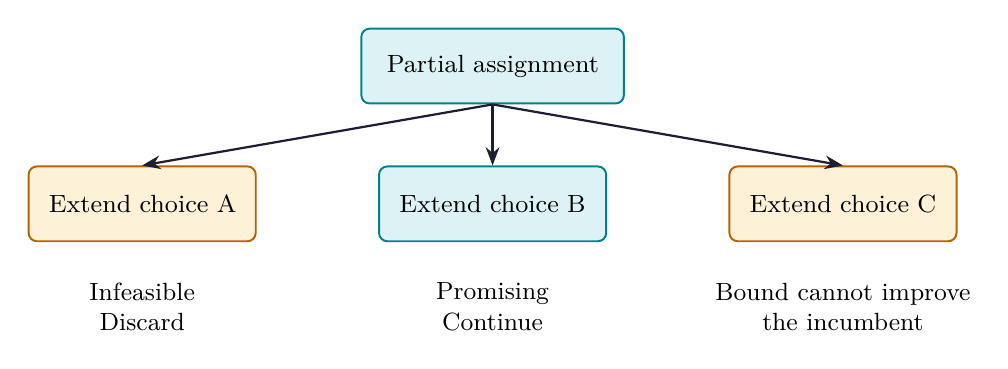
\begin{tikzpicture}[every node/.style={font=\small}]
\node[block,text width=3.1cm] (root) at (0,2.9) {Partial assignment};
\node[amberblock,text width=2.65cm] (left) at (-4.45,1.15) {Extend choice A};
\node[block,text width=2.65cm] (mid) at (0,1.15) {Extend choice B};
\node[amberblock,text width=2.65cm] (right) at (4.45,1.15) {Extend choice C};
\draw[arrow] (root.south) -- (left.north);
\draw[arrow] (root.south) -- (mid.north);
\draw[arrow] (root.south) -- (right.north);
\node[align=center] at (-4.45,-0.16) {Infeasible\\Discard};
\node[align=center] at (0,-0.16) {Promising\\Continue};
\node[align=center] at (4.45,-0.16) {Bound cannot improve\\the incumbent};
\end{tikzpicture}\par
\end{tcolorbox}

\par\vspace{5pt}
\begingroup
\setlength{\extrarowheight}{1pt}
\noindent\begin{tabularx}{\linewidth}{|B{3.55cm}|Y|Y|}
\hline
\textbf{Method} & \textbf{Tests before descending} & \textbf{Typical traversal} \\ \hline
Backtracking & Can this prefix still satisfy every constraint? & Depth-first with a recursion stack. \\ \hline
Branch-and-bound & Can any feasible completion beat the incumbent? & Depth-first, breadth-first or best-bound with a priority queue. \\ \hline
Brute force & Only the completed candidate is checked in the simplest method. & Enumerate the full candidate space. \\ \hline
\end{tabularx}\par
\endgroup
\begin{tcolorbox}[formulabox, title={Safe objective pruning}]
For minimisation, discard a node when its lower bound is at least the incumbent cost. For maximisation, discard it when its upper bound is at most the incumbent value. These comparisons find one optimum. Retain equality if every optimal solution must be listed.
\end{tcolorbox}

\begin{tcolorbox}[examplebox, title={Backtracking for subset sum}]
For nonnegative items $(3,5,6)$ and target $8$, branch on taking or skipping each item. From prefix $(3,5)$ the sum is $8$ and a valid subset is found. The prefix $(3,6)$ has sum $9$ and can be pruned, because further nonnegative items cannot reduce it. A partial sum plus the sum of all remaining items below $8$ also permits pruning. If negatives are allowed, these two bounds require modification.
\end{tcolorbox}

Both searches may still visit exponentially many nodes. A good branching order may find a strong incumbent early, but it does not change the exactness argument.

\section{Bin Packing, Knapsack and Travelling Salesperson}
Bin packing minimises the number of bins, knapsack maximises selected value under a capacity, and TSP minimises the cost of a complete tour.
\subsection{Bin packing and placement heuristics}
\begin{tcolorbox}[defbox, title={One-dimensional bin packing}]
Each item has a positive size at most the bin capacity $C$. Pack all items using the fewest bins, ensuring the total size assigned to each bin is at most $C$. The number of bins is the objective, while item placement is the decision.
\end{tcolorbox}

\begin{itemize}[leftmargin=*, itemsep=3pt, topsep=4pt]
  \item \textbf{Next Fit.} Try only the current bin. Open a new one when the item does not fit.
  \item \textbf{First Fit.} Scan bins in opening order and choose the first with enough space.
  \item \textbf{Best Fit.} Choose the feasible bin with the smallest remaining capacity after placement.
  \item \textbf{First Fit Decreasing (FFD).} Sort all sizes from largest to smallest, then use First Fit. Reordering requires access to the complete input.
\end{itemize}
\begin{tcolorbox}[examplebox, title={Trace and optimality check with capacity 10}]
The input is $(4,4,6,6)$. First Fit places the two $4$s together, then opens a bin for each $6$. FFD processes $(6,6,4,4)$ and pairs each $6$ with a $4$. Since the total size is $20$, the volume lower bound is $\lceil20/10\rceil=2$. FFD attains that bound in this instance.
\end{tcolorbox}

An exact depth-first search tries placing the next item in any bin where it fits, or opening a new one. Equivalent placements in bins with equal free space can be skipped: swapping those bins maps completions one-to-one. For minimisation, a bound is
\[
b+\left\lceil \frac{\max(0,R-F)}{C}\right\rceil,
\]
where $b$ bins are already open, $F$ is their combined free space and $R$ is the total size still unpacked. Even when pieces cannot fill $F$ perfectly, this estimate is safely optimistic.

\subsection{Fractional and zero-one knapsack}
\begin{tcolorbox}[defbox, title={Knapsack variants}]
Select items of weights $w_i>0$ and nonnegative values $v_i$ subject to capacity $W$. Fractional knapsack allows any portion of each item and scales value proportionally. Zero-one knapsack requires taking an item whole or leaving it.
\end{tcolorbox}

\begin{tcolorbox}[examplebox, title={Why density is exact for fractional knapsack}]
Order by $v_i/w_i$. If a solution takes some lower-density weight while higher-density weight is still available, swap equal amounts of those weights. The total weight is unchanged and the value cannot decrease. Repeating the exchange yields a solution with whole items in density order and at most one partially selected final item. Sorting and scanning take $O(n\log n)$ time.
\end{tcolorbox}

For capacity $50$ and items $(w,v)=(10,60),(20,100),(30,120)$, the density order is $6,5,4$. The fractional value is $60+100+(20/30)120=240$. The corresponding whole-item greedy rule takes items 1 and 2 for value $160$. Items 2 and 3 attain $220$, so the greedy rule is not exact for this zero-one instance.
\begin{tcolorbox}[formulabox, title={Zero-one recurrence and complexity}]
For positive integer weights, let $D[i,c]$ be the best value from the first $i$ items with capacity $c$. Start with $D[0,c]=0$. For $i\ge1$,
\[
D[i,c]=
\begin{cases}
D[i-1,c], & c<w_i,\\
\max\{D[i-1,c],v_i+D[i-1,c-w_i]\}, & c\ge w_i .
\end{cases}
\]
Every feasible optimum either excludes or includes the last item, which proves the two alternatives. The $O(nW)$ time bound is pseudo-polynomial because $W$ may be exponential in its binary encoding length. The full table uses $O(nW)$ space.
\end{tcolorbox}

\begin{tcolorbox}[examplebox, title={Fill a small DP and recover the selection}]
Let $(w,v)=(2,3),(3,4),(4,5)$ and $W=5$.
\par\vspace{5pt}
\begingroup
\setlength{\extrarowheight}{1pt}
\noindent\begin{tabularx}{\linewidth}{|B{2.55cm}|Y|Y|Y|Y|Y|Y|}
\hline
\textbf{Capacity} & \textbf{0} & \textbf{1} & \textbf{2} & \textbf{3} & \textbf{4} & \textbf{5} \\ \hline
No items & 0 & 0 & 0 & 0 & 0 & 0 \\ \hline
Item 1 & 0 & 0 & 3 & 3 & 3 & 3 \\ \hline
Items 1--2 & 0 & 0 & 3 & 4 & 4 & 7 \\ \hline
Items 1--3 & 0 & 0 & 3 & 4 & 5 & 7 \\ \hline
\end{tabularx}\par
\endgroup
At $(3,5)$ the value is unchanged from row 2, so item 3 can be skipped. At $(2,5)$, $4+D[1,2]=7$ improves on skipping item 2. The remaining capacity is 2 and item 1 completes the optimum.
\end{tcolorbox}

With one array, process capacities from $W$ down to $w_i$ for each item. Then $D[c-w_i]$ is still from the previous row when $D[c]$ is updated. Ascending iteration can reuse item $i$ within the same round. One-row memory is $O(W)$ for computing the value.
\begin{tcolorbox}[examplebox, title={A fractional upper bound in zero-one branch-and-bound}]
In the capacity-$50$ instance, first obtain a feasible incumbent of value $220$ using items 2 and 3. On the branch that includes item 1 and excludes item 2, at most $40$ capacity remains and only item 3 is available. Its fractional relaxation gives $60+120=180$. Prune the branch. On the branch excluding item 1, the upper bound is $220$. On the branch containing items 1 and 2, item 3 is infeasible as a whole, so its best complete value is $160$. This covers every branch and proves $220$ optimal.
\end{tcolorbox}

\subsection{Travelling salesperson problem and route design}
\begin{tcolorbox}[defbox, title={Travelling salesperson problem (TSP)}]
Given a distance or cost for travelling between cities, find a least-cost tour that starts at one city, visits every other city exactly once, and returns to the start. Distances may be symmetric. A \textbf{metric} TSP additionally obeys the triangle inequality.
\end{tcolorbox}

\begin{itemize}[leftmargin=*, itemsep=3pt, topsep=4pt]
  \item \textbf{Brute force.} Fix the starting city, enumerate permutations and include the return edge in every cost.
  \item \textbf{Backtracking.} Extend the route with an unvisited city. Reject an illegal edge or a move that would repeat a city.
  \item \textbf{Branch-and-bound.} For a symmetric instance and a nonempty unvisited set $U$, add three terms to the prefix cost: an MST on $U$, the cheapest edge from the current endpoint to $U$, and the cheapest edge from $U$ back to the start. Every completion contains such a connection at both ends and a spanning path through $U$. If $U$ is empty, add the actual return edge.
  \item \textbf{Heuristic.} Nearest neighbour chooses the cheapest edge to an unvisited city. A local improvement such as 2-opt replaces two tour edges by reversing a segment when the symmetric tour becomes shorter.
\end{itemize}
\begin{tcolorbox}[formulabox, title={Held--Karp subset DP}]
Fix start $s$ and use $D[S,j]$ for the cheapest path from $s$ visiting exactly the other cities in nonempty $S$, ending at $j\in S$. Then
\begin{align*}
D[\{j\},j]&=c(s,j),\\
D[S,j]&=\min_{i\in S\setminus\{j\}}\{D[S\setminus\{j\},i]+c(i,j)\}.
\end{align*}
The recurrence examines every possible penultimate city. With $U$ equal to all non-start cities, close the tour using $\min_{j\in U}(D[U,j]+c(j,s))$. Time is $O(n^2 2^n)$ and space is $O(n2^n)$. Store the minimising predecessor to recover the tour.
\end{tcolorbox}

\begin{tcolorbox}[examplebox, title={Four-city TSP and a greedy counterexample}]
Let the symmetric edge costs be $AB=10$, $AC=15$, $AD=20$, $BC=35$, $BD=25$ and $CD=30$. From start $A$, the three tours up to reversal cost
\begin{align*}
A\!-\!B\!-\!C\!-\!D\!-\!A &: 10+35+30+20=95,\\
A\!-\!B\!-\!D\!-\!C\!-\!A &: 10+25+30+15=80,\\
A\!-\!C\!-\!B\!-\!D\!-\!A &: 15+35+25+20=95.
\end{align*}
Nearest neighbour from $A$ gives cost $80$. From $D$ it chooses $D,A,B,C,D$ for $95$. The result can depend on the start.
\par
\textbf{Trace one Held--Karp state.} With start $A$, the path to $D$ through $C$ costs $15+30=45$. The path to $C$ through $D$ costs $20+30=50$. To end at $B$ after visiting all three cities, compare the two penultimate cities:
\[
\begin{aligned}
D[\{B,C,D\},B]&=\min\{50+35,\ 45+25\}\\
               &=70.
\end{aligned}
\]
The paths ending at $C$ and $D$ have costs $65$ and $75$. After adding the return edges, the candidates are $80$, $80$ and $95$. The optimal tour has cost $80$.
\end{tcolorbox}

\subsection{Heuristic characteristics and application domains}
\begin{tcolorbox}[defbox, title={Heuristic}]
A \textbf{heuristic} is a practical rule for finding good feasible solutions with limited time or memory. Results can depend on input order, tie-breaking and starting point. An approximation algorithm adds a proved quality guarantee.
\begin{itemize}[leftmargin=*, itemsep=1pt, topsep=2pt]
  \item \textbf{Packing.} Use First Fit for placement. Compare bin count with a lower bound.
  \item \textbf{Routing.} Use nearest neighbour and 2-opt. Compare tour costs across starts.
  \item \textbf{Scheduling.} Rank jobs by urgency. Check lateness and missed deadlines.
\end{itemize}
\end{tcolorbox}

\newpage
\begin{center}
  {\large\bfseries\color{myred} Quick Revision --- Module 2}\\[3pt]
  {\small\color{mydark} Algorithm Design Strategies $|$ ES-CS401}
\end{center}
\noindent{\color{myred}\rule{\linewidth}{1.2pt}}\par\vspace{4pt}

\begin{tcolorbox}[formulabox, title={Key Concepts at a Glance}]
\renewcommand{\arraystretch}{1.35}
\noindent\begin{tabularx}{\linewidth}{B{4.5cm}Y}
Brute force & $2^n$ subsets or $(n-1)!$ fixed-start orders before symmetry reductions. \\[3pt]
Bin packing lower bound & $\lceil\sum_i s_i/C\rceil$ by total volume. \\[3pt]
Knapsack DP & $O(nW)$ time for integer capacity $W$, pseudo-polynomial. \\[3pt]
TSP subset DP & $O(n^2 2^n)$ time and $O(n2^n)$ space. \\[3pt]
Bound directions & Minimisation uses a lower bound on a node. Maximisation uses an upper bound. \\[3pt]
\end{tabularx}\par
\end{tcolorbox}

\begin{tcolorbox}[defbox, title={One-Line Definitions}]
\begin{itemize}[leftmargin=*, itemsep=3pt, topsep=4pt]
  \item \textbf{Greedy choice.} A locally preferred decision committed under a fixed rule.
  \item \textbf{Incumbent.} The best complete feasible solution found so far.
  \item \textbf{State-space tree.} A tree whose branches extend a partial assignment.
  \item \textbf{Heuristic.} A practical search or selection rule whose quality can depend on the instance.
\end{itemize}
\end{tcolorbox}

\begin{tcolorbox}[exambox, title={Frequently Asked / Viva Questions}]
\begin{enumerate}[topsep=0pt, label=\textbf{Q\arabic*.}, itemsep=5pt, leftmargin=*]
  \item \Q{Why is exhaustive search correct?}
    It examines every possible optimum before choosing the best feasible candidate.
  \item \Q{How do exchange arguments work?}
    Replace a choice in an optimum by a greedy one without loss, then repeat on the remaining instance.
  \item \Q{What makes DP useful?}
    Smaller states determine larger ones, and storing repeated states avoids duplicate work.
  \item \Q{How does memoisation differ from tabulation?}
    Memoisation follows recursive dependencies on demand. Tabulation uses an explicit dependency order.
  \item \Q{Why must one-row zero-one DP run backward?}
    It avoids selecting the new item multiple times during the same iteration.
  \item \Q{Why is fractional knapsack useful inside branch-and-bound?}
    It relaxes the restrictions and provides an upper bound on achievable value.
  \item \Q{What does backtracking prune?}
    A prefix that cannot lead to any feasible completion.
  \item \Q{What does branch-and-bound prune?}
    A subtree whose optimistic value cannot improve the incumbent.
  \item \Q{Which packing rule requires the whole input?}
    First Fit Decreasing sorts sizes before placing items.
  \item \Q{What edge is easy to forget in TSP?}
    The return edge from the last visited city to the start.
  \item \Q{What is a safe way to assess a heuristic?}
    Check feasibility, solution value, runtime and comparisons against lower bounds or exact small cases.
\end{enumerate}
\end{tcolorbox}

\begin{tcolorbox}[tikzbox, title={Summary Comparison}]
\par\vspace{5pt}
\begingroup
\setlength{\extrarowheight}{1pt}
\noindent\begin{tabularx}{\linewidth}{|B{3.45cm}|Y|Y|}
\hline
\textbf{Strategy} & \textbf{Main condition or mechanism} & \textbf{Typical use} \\ \hline
Greedy & Safe choices established by an exchange or cut proof. & Interval scheduling and fractional knapsack. \\ \hline
Dynamic programming & A tractable collection of reusable states. & Integer knapsack and subset TSP. \\ \hline
Backtracking & Constraint-based pruning. & Feasible subsets and route enumeration. \\ \hline
Branch-and-bound & Objective-based pruning with an incumbent. & Exact packing, knapsack and TSP. \\ \hline
\end{tabularx}\par
\endgroup
\end{tcolorbox}

\end{document}
